\section{Benachrichtigungsservice}
\label{notifications}
% die Idee dahinter
Die Idee hinter dem Benachrichtigungsservice ist, dass die Benutzer per Mail informiert werden, sobald der von ihnen definierte Grenzwert über- bzw. unterschritten wird. Dies kann zum Beispiel ein Segler sein, der wissen möchte, wann genügend Wind vorhanden ist, oder ein Bootsbesitzer, der wissen will, wann der Pegel unter einen bestimmten Wert fällt.


%% ############################################################################
%% Unterkapitel
%% ############################################################################
\subsection{Funktionsprinzip des Benachrichtigungsservices}

Der Benachrichtigungsservice ist so aufgebaut, dass auf der Webseite ein Formular mit den gewünschten Daten ausgefüllt werden kann. Das Ganze funktoniert ohne Benutzeraccount. In Abbildung\,\ref{img:notificationKonzept} ist der Ablauf grafisch dargestellt: Der Benutzer füllt ein Formular aus, dessen Daten per \emph{POST}-Befehl an den Server gesendet werden. Der Server speichert die Daten zusammen mit einem eindeutigen Schlüssel (Hash) in der Datenbank. Damit sichergestellt ist, dass derjenige, dessen E-Mail-Adresse angegeben wurde, auch wirklich der Besteller ist, muss der Benachrichtiungsservice zuerst aktiviert werden. Der Server sendet dazu ein Mail mit dem Aktivierungslink an die genannte E-Mail-Adresse. Erst wenn dieser Link aufgerufen wurde, ist der entsprechende Service aktiv. Da es keinen Benutzeraccount gibt, wird in jedem Mail, das versendet wird, ein Unsubscribe-Link mitgeschickt. So kann der Benutzer den Service selbständig wieder löschen.

\begin{figure}[h!]
  \fbox{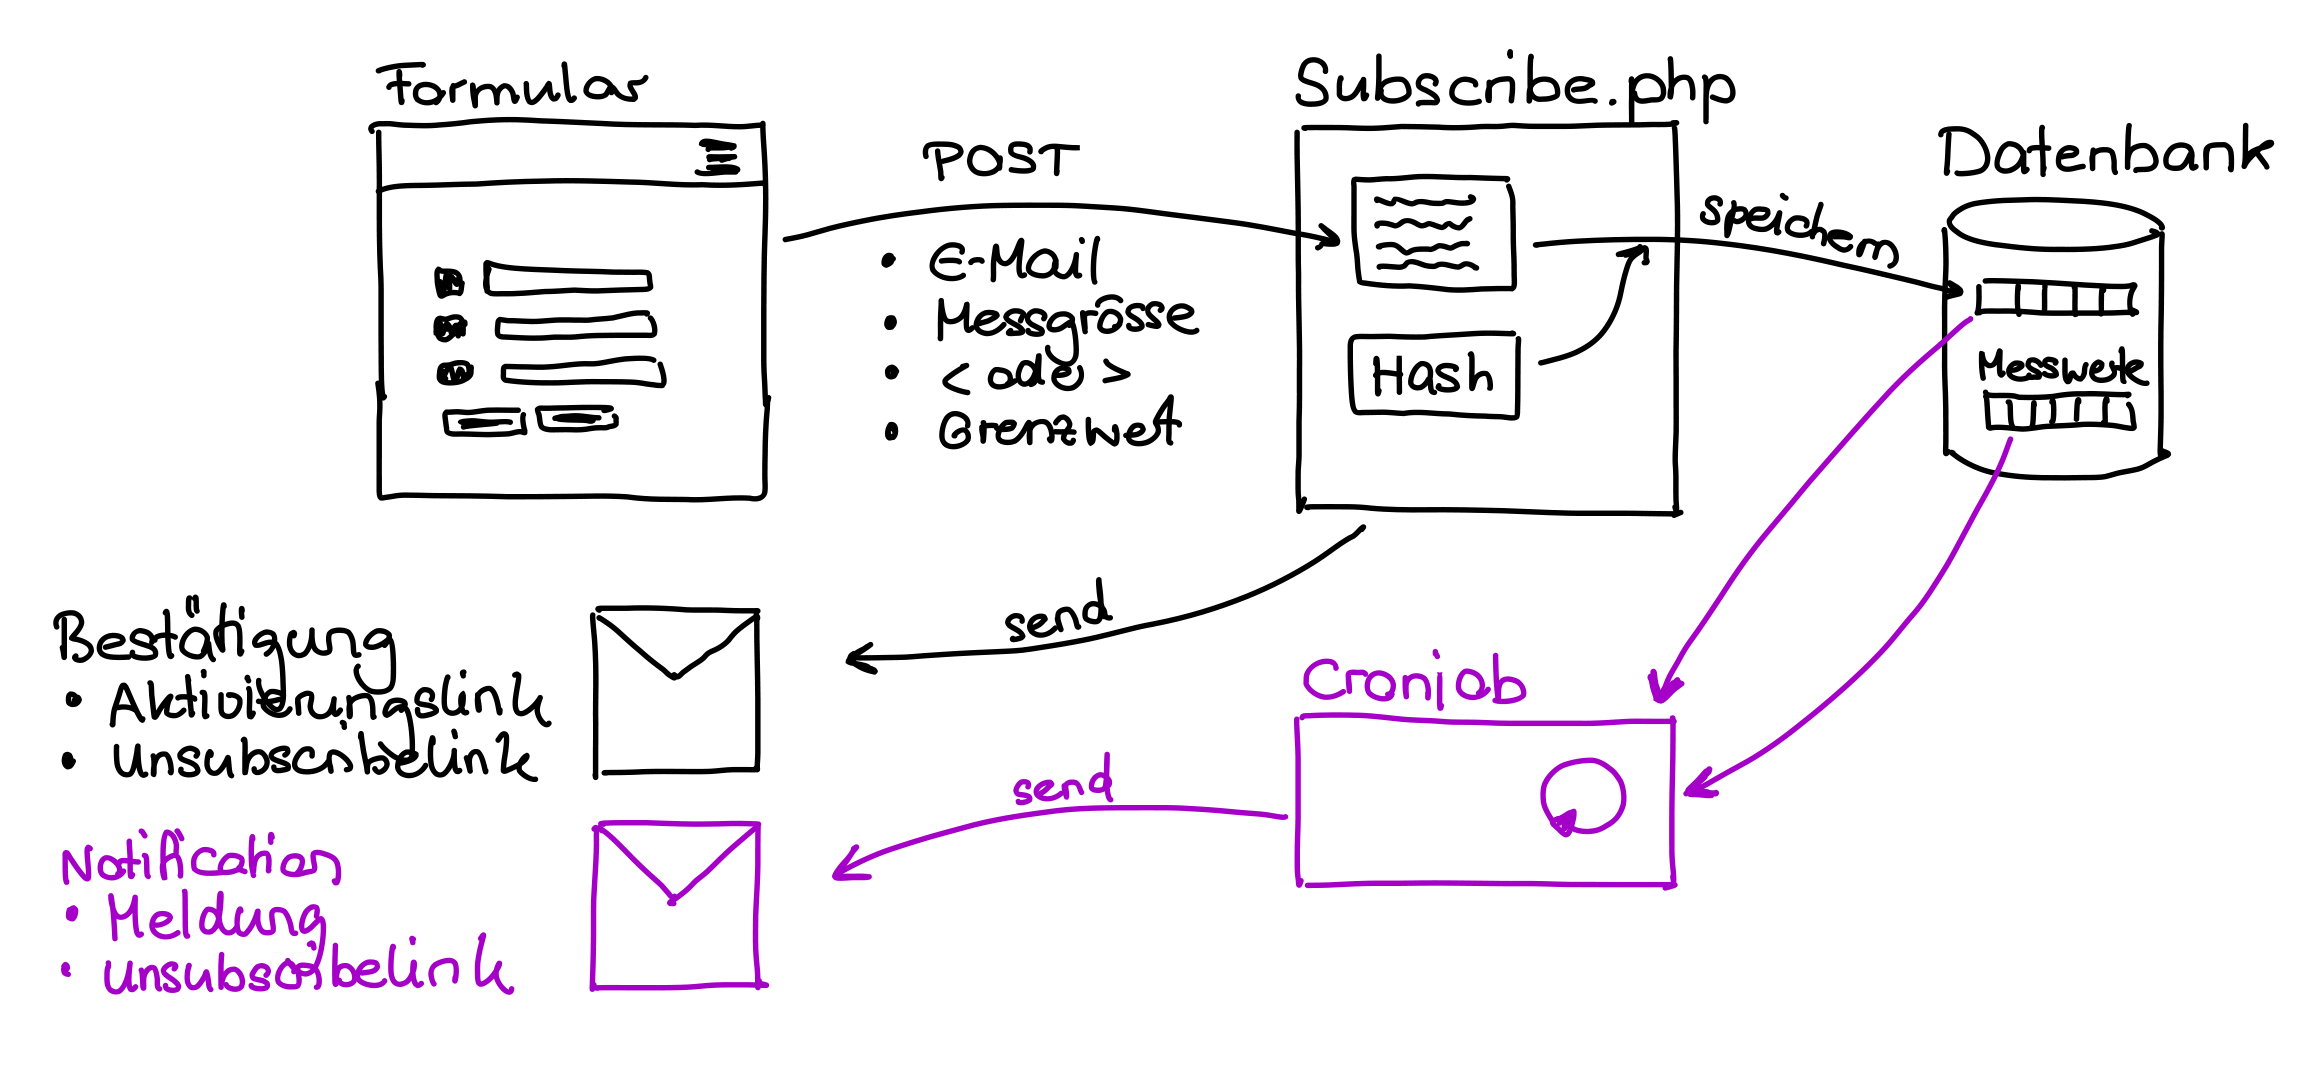
\includegraphics[width=\textwidth-2\fboxsep-2\fboxrule]{img/notificationKonzept}}
	\centering
	\caption{Funktionsprinzip des Benachrichtigungsservices}
	\label{img:notificationKonzept}
\end{figure}

\noindent
Der Benachrichtigungsservice selbst basiert auf einem Cronjob, der einmal pro Stunde läuft. Das Prinzip ist in Abbildung\,\ref{img:notificationKonzept} in violett dargestellt. Der Cronjob ruft sämtliche Einträge in der Notification-Tabelle ab und vergleicht sie mit den Messwerten. Sobald eine Bedingung erfüllt ist, wird ein Benachrichtigungs-Mail an die hinterlegte E-Mail-Adresse gesendet. Neben der eigentlichen Meldung ist ein Unsubscribe-Link vorhanden, damit der Benutzer den Benachritigungsservice abbestellen kann.

%% ############################################################################
%% Unterkapitel
%% ############################################################################
\subsection{Formular mit integrierter Überprüfung der Eingabe}
Das Formular des Benachrichtigungsservices besteht aus vier Eingabe- bzw. Auswahlfeldern, wie in Abbildung\,\ref{img:notificationFE} links dargestellt. Zuoberst kann die gewünschte Messgrösse ausgewählt werden. Das Dropdown-Menü stellt sicher, dass nur Werte ausgewählt werden können, die von der Wetterstation zur Verfügung gestellt werden. Mit den Radio-Buttons kann ausgewählt werden, ob der Messwert grösser oder kleiner als der Grenzwert sein soll. Der Grenzwert wird als Zahl eingeben auf eine Stelle nach dem Komma genau. Zuletzt muss die E-Mail-Adresse, an welche die Benachrichtigung gesendet werden soll, eingetragen werden. Durch Anklicken des Abonnieren-Buttons wird das Formular abgesendet.

\begin{figure}[htbp!]
  \fbox{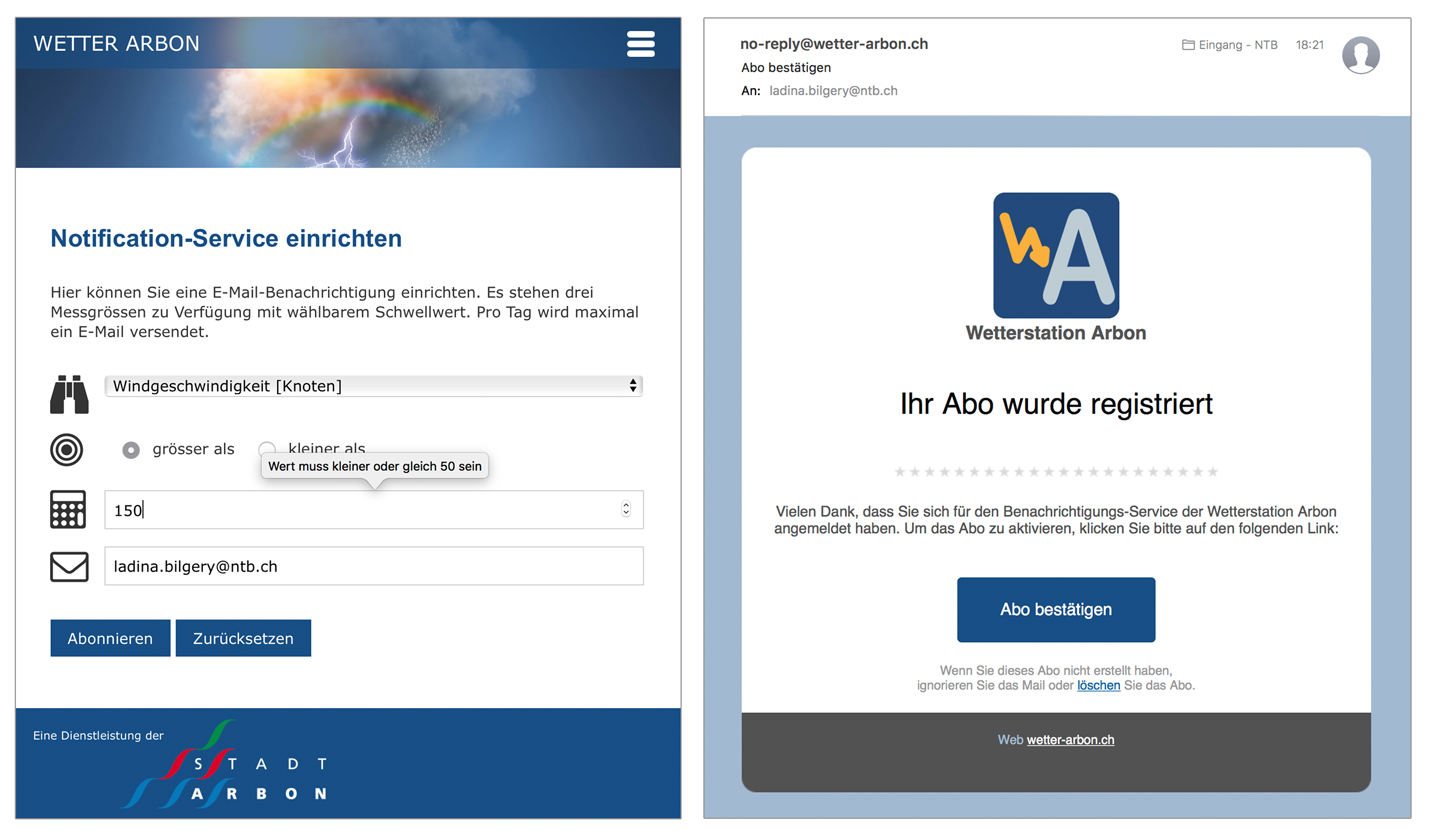
\includegraphics[width=\textwidth-2\fboxsep-2\fboxrule]{img/notificationFE2}}
	\centering
	\caption{Eingabeüberprüfung und E-Mail-Design des Benachrichtigungsservices}
	\label{img:notificationFE}
\end{figure}

\noindent
Bisher musste die clientseitige Formularüberprüfung manuell programmiert bzw. eine JavaScript-Bibliothek verwendet werden. Unter HTML5 ist die Formularüberprüfung direkt in die Formularfelder integriert. Über die Defintion des \emph{type} (\emph{radio}, \emph{number}, \emph{email}, \dots) und gegebenenfalls einiger Zusatzangaben, wird die Überprüfung automtisch beim Absenden des Formulars durchgeführt. Ist die Eingabe fehlerhaft, so wird dies dem Benutzer direkt angezeigt. Der Wertebereich auf unsere Webseite ist zum Beispiel eingeschränkt auf Zahlen von 1 bis 50, wie in Listing\,\ref{lst:HTML5form}, Zeile\,11, ersichtlich. Wird nun ein Wert ausserhalb dieses Bereichs eingegeben, so erhält der Benutzer eine Fehlermeldung, siehe Abbildung\,\ref{img:notificationFE} links. Das Formular wird in diesem Fall nicht abgesendet. Weiter kann angegeben werden, ob ein Feld Pflicht ist (durch die Option \emph{required}) beziehungsweise ob zum Beispiel beim Dropdown-Menü eine Auswahl ungültig ist (durch die Option \emph{disabled}).

% Überprüfung der Eingaben
\vspace{3mm}
\begin{lstlisting}[label=lst:HTML5form,caption=Integrierte Formularüberprüfung mit HTML5, language=HTML5, style=htmlcssjs]
<!-- Auswahlmenue -->
<select name="measurand" required>
  <option value="" disabled selected>Messgrösse auswählen</option>
  <option value="windspeed">Windgeschwindigkeit</option>
</select>

<!-- Radio Button -->
<input type="radio" value="greater" checked>

<!-- Zahlenbereich -->
<input type="number" min="1" step="0.1" max="50" value="6">

<!-- E-Mail Adresse -->
<input type="email" placeholder="max.mustermann@web.ch" required>
\end{lstlisting}
\vspace{3mm}

%% ############################################################################
%% Unterkapitel
%% ############################################################################
\subsection{Identifikation des Abos via URL}
Die Tabelle für die Speicherung der Abos in der Datenbank enthält neben den vom Benutzer eingegebenen Daten noch weitere Einträge. Dies ist einerseits der Status des Abos, d.h. aktiv oder inaktiv und der Zeitstempel des letzen Mails, damit maximal einmal pro Tag ein Mail versendet wird, andererseits ist dies der eindeutige, nicht erratbare Schlüssel (Hash), welcher für sämtliche Datenbank-Operationen benötigt wird. Der Hash wird erzeugt, indem zuerst eine Zufallszahl zwischen 0 und 1000 generiert wird und danach mit dem SHA-256-Algorithmus der Hash daraus berechnet wird (Listing\,\ref{lst:randomHash}).

\vspace{3mm}
\begin{lstlisting}[label=lst:randomHash,caption=Funktion zur Erzeugung des eindeutigen Hash, language=php, style=php]
$hash = hash("sha256",rand(0,1000));
// Beispiel: Input = 689; Output =
// fc4fb94d36f45aa9d13358022455e55db4b6f0eb536a1b2897c90dfd3df9eb9b

\end{lstlisting}
\vspace{3mm}

\noindent
Es gibt insgesamt drei verschiedene Befehle, die der Browser dem Server senden kann. Der Erste ist die Bestellung des Abos (\textit{subscribe}). Dies erfolgt automatisch, sobald das Formular abgesendet wird. Der Zweite ist die Verifizierung der E-Mail-Adresse (\textit{verify}) und als letztes die Löschung des Abos (\textit{unsubscribe}). Erstere ist eine POST-Meldungen, die beiden anderen eine GET-Meldung, wobei die URL jeweil zur Identifizierung des Abos die E-Mail-Adresse und den Schlüssel (Hash) des entsprechenden Abos enthält. Der Link für die Aktivierung des Abos lautet beispielhaft wie in Listing \ref{lst:verify} aufgeführt.

\vspace{3mm}
\begin{lstlisting}[label=lst:verify,caption=Beispiellink für die Aktivierung eines Abos, language=HTML5, style=htmlcssjs]
https://dev.wetter-arbon.ch/application/php/verify.php?
email=ladina.bilgery@ntb.ch&
hash=81f27f8a7d8766c72c0307a31327c1fad9007c6c3d33724ad2a5c0a8fe0df33d
\end{lstlisting}
\vspace{3mm}

\noindent
Auf diese Weise kann auf Grund der aufgerufen Seite (\textit{subscribe.php}, \textit{verify.php}, \textit{unsubscribe.php}) und dem Paar E-Mail und Hash die Datenbankoperation genau definiert werden.

%% ############################################################################
%% Unterkapitel
%% ############################################################################
\subsection{Design des Benachrichtigungs-Mails}
Das Benachrichtigungs-E-Mail wird als sogenanntes \emph{MIMEMultipart}-Mail versendet. Das heisst, es enthält einerseits einen unformatierten Plaintext und andererseits eine mit Grafiken und Farben versehene HTML-Version. Verwendet wird dazu die Python-Bibliothek \emph{smtplib}. Zur Erzeugung des Layouts des HTML-Emails kam die kostenlose Version des Online-Tools \emph{\href{https://beefree.io/bee-free/}{BEEfree}} zum Einsatz. Das E-Mail-Layout ist in Abbildung\,\ref{img:notificationFE} rechts dargestellt.



%Als Absenderadresse wurde \emph{no-reply@wetter-arbon.ch} gewählt, um dem Benutzer zu informieren, dass dies keine Kontakt-E-Mail-Adresse ist.
